% !TeX spellcheck = cs_CZ
\wikitextrule
\begin{example}\label{FYZ:exam005}
  Spočtěte, jakou vzdálenost v metrech vyjadřuje jeden parsek \protect\cite[s.~3]{Kulhanek2009}.
  
  \textbf{Řešení}: \(\SI{1}{\parsec}\) (paralaktická sekunda) je vzdálenost, ze které vidíme 
  velkou poloosu oběžné dráhy Země kolem Slunce pod uhlem \(\varphi = \ang{;;1}\). Úhel 
  \(\ang{;;1}\) je tak malý, že strany \(VS\) a \(VZ\) na obrázku prakticky splývají a místo 
  pravého trojúhelníka $VSZ$ můžeme použít definiční vztah úhlu v obloukové míře (\emph{velkost 
  úhlu je možné určit jako poměr délky oblouku vymezeného rameny na kružnici opsané kolem 
  vrcholu k poloměru této kružnice}). Proto 
  
   {\centering
    \captionsetup{type=figure}
    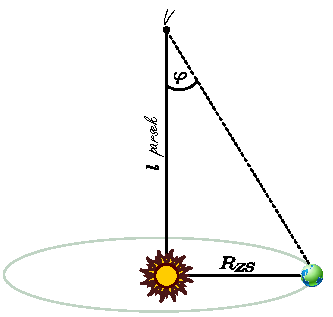
\includegraphics[width=0.6\linewidth]{fyz_fig224.pdf}
    \captionof{figure}[Parsek]{K příkladu \ref{FYZ:exam005}: Odvození velikosti Parseku}
    \label{fyz:fig224}
    \par}
  \begin{equation*}
    \varphi = \frac{R_{SZ}}{l} \rightarrow l = \frac{R_{SZ}}{\varphi},
  \end{equation*}
  kde $l$ je vzdálenost \SI{1}{\parsec} v metrech, $R_{SZ}$ je vzdálenost země od Slunce a 
  $\varphi$ je úhel jedné vteřiny vyjádřený v radiánech. 
  \begin{equation*}
      l = \frac{\SI{1.5e11}{\meter}}{\dfrac{1}{60\cdot60} 
          \cdot\dfrac{2\pi}{360}}\cong \SI{3e16}{\meter}.
  \end{equation*}
\end{example}
\wikitextrule